\documentclass[border=0.5in]{blog}

\usepackage{hyperref}
\usepackage{listings}
\usepackage{natbib}
\usepackage{subfigure}

\usepackage{tikz}
\usepackage{pgfplots}
\usetikzlibrary{arrows,shapes,snakes,automata,backgrounds,petri,matrix}
\tikzstyle{brick} = [rectangle, minimum height = 0.7cm, text centered, draw = black]
\newcommand\xaxis{210}
\newcommand\yaxis{-30}
\newcommand\zaxis{90}
\newcommand\topside[3]{
    \fill[fill=yellow, draw=black,shift={(\xaxis:#1)},shift={(\yaxis:#2)},
    shift={(\zaxis:#3)}] (0,0) -- (30:1) -- (0,1) -- (150:1) -- (0,0);
}
% The left side of a cube
\newcommand\leftside[3]{
    \fill[fill=red, draw=black,shift={(\xaxis:#1)},shift={(\yaxis:#2)},
    shift={(\zaxis:#3)}] (0,0) -- (0,-1) -- (210:1) --(150:1)--(0,0);
}
% The right side of a cube
\newcommand\rightside[3]{
    \fill[fill=green, draw=black,shift={(\xaxis:#1)},shift={(\yaxis:#2)},
    shift={(\zaxis:#3)}] (0,0) -- (30:1) -- (-30:1) --(0,-1)--(0,0);
}
% The cube 
\newcommand\cube[3]{
    \topside{#1}{#2}{#3}
    \leftside{#1}{#2}{#3}
    \rightside{#1}{#2}{#3}
}

\usepackage{amsmath}

\title{OctNet: Efficient Operations and Data Structure}
\author{Johann Lee \\ me@qinka.pro}
\date{Dec. 12, 2017}


\begin{document}
    \maketitle
    \begin{abstract}
        I write this post to review the paper:
        \citep{DBLP:journals/corr/RieglerUG16}\textit{OctNet: Learning Deep 3D Representation at High Resolutions}.
    \end{abstract}

    \begin{license}
        \copyleft{2018}{Johann Lee <me@qinka.pro>}
        
        \par Permission is granted to copy, distribute and/or modify this document
        under the terms of the GNU Free Documentation License, Version 1.3
        or any later version published by the Free Software Foundation;
        with no Invariant Sections, no Front-Cover Texts, and no Back-Cover Texts.
        A copy of the license is included in the section entitled "GNU
        Free Documentation License".
    \end{license}

    \tableofcontents

    \section{Related works, Background, and Motivation}
    \label{sec:rbm}
    
    In this section, I will talk about the related works, backgrounds and the motivations of 3-D deep learning using octree-based Convolutional Neural Network.\citep{DBLP:journals/corr/RieglerUG16}
    
    \subsection{[Related works] 2-D Images based CNN}
    \label{sec:rbm:2dcnn}
    
    CNN has made a great success in 2-D image deep learning.
    
    In the rent few years, CNN had become the workhorse in computer vision.
    When people do researches in computer vision, ConvNet and its operations
    are necessary. With more efficient learning and less parameters,
    CNN is the best tools.
    And when searching key word ``CNN'' on \url{arxiv.org} the numbers of results 
    is more than 1000.
    
    \paragraph{\citep{DBLP:journals/corr/FlynnNPS15}}
    
    In the paper (2015)\textit{DeepStereo: Learning to Predict New Views from the World’s Imagery}, authors present a novel network to analyze the images.
    The basic point of what they want to do is to generate image from the difference views of
    a same scene. The fig.\ref{fig:DeepStereo} is the example from  the paper.
    \begin{figure}
        \centering
        \subfigure[Synthesized result]{
            \includegraphics[width=0.7\linewidth]{../../../image/DeepStereo}
            \label{fig:DeepStereo:o}
        }
    
        \subfigure[Training input 1]{\
            \includegraphics[width=0.35\linewidth]{../../../image/DeepStereo-1}
            \label{fig:DeepStereo:i1}
        }
        \subfigure[Training input 2]{
            \includegraphics[width=0.35\linewidth]{../../../image/DeepStereo-2}
            \label{fig:DeepStereo:i2}
        }
        \caption{Use the different views of a scene to generate new image.}
        \label{fig:DeepStereo}
    \end{figure}
    
    \paragraph{\citep{DBLP:journals/corr/GhiasiF16}}
    
    This paper point a problem of relying on spatial pooling which makes it difficult to adapt them to the tasks with dense, pixel-accurate labeling.
    First thing they do is
    \begin{quote}
        Demonstrate that while the apparent spatial resolution of convolutional feature maps is low, the high-dimensional feature repre- sentation contains significant sub-pixel localization information.
    \end{quote}
    And the second thing they do is
    \begin{quote}
        Describe a multi-resolution reconstruction architecture based on a Lapla- cian pyramid that uses skip connections from higher resolution feature maps and multiplicative gating to successively refine segment bound- aries reconstructed from lower-resolution maps.
    \end{quote}

    \paragraph{\citep{DBLP:journals/corr/HeZRS15}}
    
    This paper present a residual learning framework to ease the training of networks that are substantially deeper. They add a ``direct link'' between 
    some of conv layers, just like \ref{fig:residual-conv-net-block}.
    
    \begin{figure}
        \centering
        \includegraphics[width=0.4\linewidth]{../../../image/residual-conv-net}
        \caption{Building block}
        \label{fig:residual-conv-net-block}
    \end{figure}
    
    \paragraph{\citep{DBLP:journals/corr/RenHG015}}
    
    In this paper, they present a Region Proposal Network, RPN for short.
    RPN can share the full-image convolutional features with the detection network.
    <TODO>
    
    \paragraph{\citep{DBLP:journals/corr/SuMKL15}}
    
    In this paper, they use the 2-D CNN and multi-view of a 3-D object to recognize
    3-D shape.
    \begin{figure}
        \centering
        \includegraphics[width=0.5\linewidth]{../../../image/multi-view}
        \caption{Multi-view of a chair.}
        \label{fig:chair-multi-view}
    \end{figure}
    The fig.\ref{fig:chair-multi-view} can be an example. They just render the many
    2-D image from the different view of a chair as the input, and then use a multi-view conv network to predicted the class of chair.
    
    \paragraph{\citep{DBLP:journals/corr/TatarchenkoDB15}}
    
    This paper use a single image and work with CNN to generate a 3-D(RGBD) object.
    For example, with single image of cup from the single view, that network can
    generate a 3-D model in RGBD of the cup. Fig.\ref{fig:generate-3-d-object} is
    its network.
    
    \begin{figure}
        \centering
        \includegraphics[width=0.7\linewidth]{../../../image/generate-3-d-object}
        \caption{The network of \citep{DBLP:journals/corr/TatarchenkoDB15}}.
        \label{fig:generate-3-d-object}
    \end{figure}
    
    \paragraph{\citep{DBLP:journals/corr/0001XLTTTF16}}
    
    This paper present a 3-D Interpreter Network, 3D-INN for short.
    The 3D-INN use a 2-D image as the input and try to work out the 2D key-points,
    and to estimate a 3D skeleton, just like the flow in fig.\ref{fig:3d-inn}.
    
    \begin{figure}
        \centering
        \includegraphics[width=0.7\linewidth]{../../../image/3D-INN}
        \caption{The network of \citep{DBLP:journals/corr/0001XLTTTF16}}.
        \label{fig:3d-inn}
    \end{figure}
    
    
    \paragraph{\citep{DBLP:journals/corr/XieGF16}}
    This paper is aimed a covert 2-D image to 3-D image.
    The 2-D image will be used as the input to a Deep3D network, and then
    the output of this network will be anaglyph 3-D image, just like fig. .
    
    \begin{figure}
        \centering
        \includegraphics[width=0.7\linewidth]{../../../image/2d-anaglyph-3d}
        \caption{The network of \citep{DBLP:journals/corr/XieGF16}}.
        \label{fig:2d-anaglyph-3d}
    \end{figure}
    
    \paragraph{\citep{DBLP:journals/corr/abs-1710-08247}}
    
    This paper is concerned with 2-D image and camera pose.
    <TODO>
    
    
    \subsection{[Motivation] Using CNN in 3-D objects}
    \label{sec:rbm:usingcnn3d}
    
    With success of CNN in 2-D images, the people begin using CNN on 3-D deep learning.
    Because of the great advantages of CNN in analyzing and learning the inner
    connections between each pixel or element of the object, CNN should also be
    the workhorse in 3-D deep learning.
    
    \subsection{[Related works] 3-D based CNN}
    \label{sec:rbm:3d-cnn}
    
    The CNN have been widely used in 2-D deep learning.
    so it's also used in 3-D deep learning.
    
    \subsubsection{Dataset: Princeton ModelNet}
    \label{sec:rbm:ds}
    
    The Princeton ModelNet dataset is a 3-D object dataset with CAD.
    
    \paragraph{Goal}
    Goal of ModelNet dataset is to provide researchers in CV, robotics, and cognitive science 
    
    \paragraph{How}
    \begin{enumerate}
        \item There is a list of the most common object categories, using the statistics obtained from SUN dataset.
        \item They hired human to label the data with their own in house designed tool with quality control.
    \end{enumerate}
    
    \paragraph{Example}
    
    The video \href{https://www.bilibili.com/video/av17197740/}{av17197740} on BiliBili
    is an example(fig.) of ModelNet with \href{https://github.com/Qinka/hOff}{hOff}.
    
    hOff is a application with OpenGL to display the model in OFF format.
    
    \begin{figure}
        \centering
        \subfigure[A table]{        \includegraphics[width=0.35\linewidth]{../../../image/modelnet-hoff-demo}
            \label{fig:modelnet-hoff-demo}}
        \subfigure[A bed]{\includegraphics[width=0.35\linewidth]{../../../image/bed_0572}
            \label{fig:bed0572}}
        \caption{Example of ModelNet}
        \label{fig:modelnet}
    \end{figure}
    
    \subsubsection{Dense Models}
    \label{sec:rbm:3d-cnn:dm}
    
    \paragraph{\citep{DBLP:journals/corr/WuSKTX14}}
    
    This paper is based on a dense model. Their model is based on the voxels.
    The data model will the translate to the voxel-represented object and then
    use the 3-D CNN to learning the data just like fig.\ref{fig:3d-shape-net}.
    
    \begin{figure}
        \centering
        \includegraphics[width=0.7\linewidth]{../../../image/3dshapenet}
        \caption{The network of \citep{DBLP:journals/corr/WuSKTX14}}.
        \label{fig:3d-shape-net}
    \end{figure}


    \paragraph{\citep{maturana_iros_2015}}
    
    This paper use the RGBD image data to recognize the objects.
    They transform the RGBD data, or points cloud to grids or voxes.
    Then they use 3-D CNN to learn the data and get the class of object.
    
    \begin{figure}
        \centering
        \includegraphics[width=0.7\linewidth]{../../../image/voxnet}
        \caption{The network of \citep{maturana_iros_2015}}.
        \label{fig:voxnet}
    \end{figure}
    
    \paragraph{\citep{DBLP:journals/corr/AlvarZB16}}
    
    This paper use the 3-D CNN with two areas:
    \begin{itemize}
        \item Classification
        \item Orientation
    \end{itemize}
    For classification, the network can distinguish different objects.
    For orientation, the network can not only do classification, but also recognize
    the direction of object.
    
    \paragraph{\citep{DBLP:journals/corr/SharmaGF16}}
    
    This paper is about the voxel-based 3-D deep learning without object labels.
    
    \paragraph{\citep{DBLP:journals/corr/BrockLRW16}}
    
    This paper is a voxel-based 3-D deep learning model.
    And it got the highest accuracy on Princeton ModelNet dataset.
    
    \paragraph{\citep{DBLP:journals/corr/GirdharFRG16}}
    
    This paper present a network that use the generated 3-D voxel data
    and 3-D rendered image of a ``real'' object as the input, and the output
    is the 3-D object.
    
    \begin{figure}
        \centering
        \includegraphics[width=0.7\linewidth]{../../../image/GirdharFRG16}
        \caption{The network of \citep{DBLP:journals/corr/GirdharFRG16}}.
        \label{fig:GirdharFRG16}
    \end{figure}


    \paragraph{\citep{DBLP:journals/corr/ChoyXGCS16}}
    In this paper, they present a novel network,
    named 3D Recurrent Reconstruction Neural Network, 3D-R$^2$N$^2$ for short.
    They use image as input, and the output is generated 3-D model from the image.
    <TODO>

    \begin{figure}
        \centering
        \includegraphics[width=0.7\linewidth]{../../../image/3d-r2n2}
        \caption{The overview of \citep{DBLP:journals/corr/ChoyXGCS16}}.
        \label{fig:3d-r2n2}
    \end{figure}
    
    \paragraph{\citep{DBLP:journals/corr/MilletariNA16}}
    
    In this paper, the authors use the fully convolutional neural networks for 
    volumetric medical image segmentation.
    <TODO>
    
    \paragraph{\citep{DBLP:journals/corr/SongX15}}
    
    In this paper, they present Deep Sliding Shapes, a 3D ConvNet formulation.
    Deep Sliding Shapes uses the RGBD data as input,
    and the output is 3D object bounding boxes.
    <TODO>
    
    \paragraph{\citep{DBLP:journals/corr/CicekALBR16}}
    
    In this paper, they transform the raw image to a manual sparse annotation,
    and then use the 3-D u-net to get dense segmentation. So they can do the segmentation.
    <TODO>
    
    
    \subsubsection{Sparse Models}
    \label{sec:rbm:3d-cnn:sm}
    
    
    \paragraph{\citep{DBLP:journals/corr/EngelckeRWTP16}}
    
    This paper use points cloud to represent 3-D objects, and detect the 
    objects with an efficient approach of natively CNN for 3-D points cloud.
    
    \begin{figure}
        \centering
        \subfigure[Example with network structure of \citep{DBLP:journals/corr/EngelckeRWTP16}]{%
            \includegraphics[width=0.4\linewidth]{../../../image/vote3deep}
            \label{fig:vote3d:s}
        }
        \subfigure[Realtime image of example]{%
            \includegraphics[width=0.4\linewidth]{../../../image/vote3deep-real}
            \label{fig:vote3d:r}
        }
        \caption{Example of Vote3Deep(\citep{DBLP:journals/corr/EngelckeRWTP16})}
        \label{fig:vote3d}
    \end{figure}
    
    \paragraph{\citep{DBLP:journals/corr/Graham14}}
    
    In this paper, author use the sparse data with CNN as online handwriting recognition.
    For the 2-D image, handwriting, is usually sparse, so to accelerate the recognition,
    they use the sparse convolutional neural network. While the number of pixel is $N^2$,
    the number of non-zero pixel is only $O(N)$.
    
    \paragraph{\citep{DBLP:journals/corr/Graham15}}
    
    In this paper, author experimented with CNNs on the 2D triangular-lattice and 3D tetrahedral-lattice.
    The key point of this paper is about sparse three-dimensional input data
    with sparse 3-D convolutional neural network.
    They work on different CNN on the different lattices,
    just like \ref{fig:sparse-3d-cnn-on-different-lattices}.
    \begin{figure}
        \centering
        \includegraphics[width=0.7\linewidth]{../../../image/sparse-3d-cnn-on-different-lattices}
        \caption{Convolution operation on different lattices.}
        \label{fig:sparse-3d-cnn-on-different-lattices}
    \end{figure}
    And their paper's convolutional operations is based on grid-like.
    <TODO>
    
    \paragraph{\citep{DBLP:journals/corr/KiefelJG15}}
    <TODO>
    
    \paragraph{\citep{DBLP:journals/corr/LiPSQG16}}
    \begin{quote}
        Building discriminative representations for 3D data has been an important task in computer graphics and computer vision research. 
    \end{quote}
    In this paper, they represent 3D spaces as volumetric fields,
    and propose a novel design that employs field probing filters to efficiently extract features from them.
    <TODO>
    
    \subsection{Background \& Motivation}
    \label{sec:rbm:bm}
    
    \subsubsection{Human and 3-D World}
    \label{sec:rbm:bm:human}
    
    We are the human living in the 3D world, so we research on 3D Deep Learning.
    
    I'm not sure how many dimension does the universe have, but I am sure that
    we, human, leave in the 3-D world.
    People's eyes can see the 3-D object, and understand what it is.
    So when we want machines to learn more about the world human living in,
    the research in 3-D Deep Learning becomes more popular.
    
    3-D objects will carry more details and informations compared with 2-D images,
    and it is more helpful to human daily life.
    
    So in a word, people 3-D Deep Learning is important.
    
    \subsubsection{Applications}
    \label{sec:rbm:bm:application}
    
    There are broad applications of 3D data:
    \begin{itemize}
        \item Robotics
        \item Augmented Reality
        \item Autonomous driving
        \item Medical Image Processing
        \item Scene recognition
        \item \dots
    \end{itemize}
    When necessary to analyze 3-D data, the 3-D deep learning is the best choice.
    
    \subsubsection{Difference between 2-D and 3-D}
    \label{sec:rbm:bm:2d-d-3d}
    
    There are two primary differences between 2-D image and 3-D object:
    \begin{itemize}
        \item For the normal operations, the complexity in computing and memory
            is different. 3-D data is $O(n^3)$, while 2-D is $O(n^2)$.
        \item The most 2-D image is dense data, while the most 3-D object used in
            3-D deep learning is sparse data.
    \end{itemize}

    \subsubsection{Sparse representation for 3-D data in 3-D deep leanring}
    \label{sec:rbm:bm:spare-r}
   
    So a primary task in 3-D deep learning is to represent 3-D object in the sparse way.
    The octree is a reasonable and efficient way to represent 3-D object.
    
    \section{OctNet}
    \label{sec:octnet}
    
    \subsection{OctNet Layers}
    \label{sec:octnet:struct}
    
    \begin{figure}
    \centering
    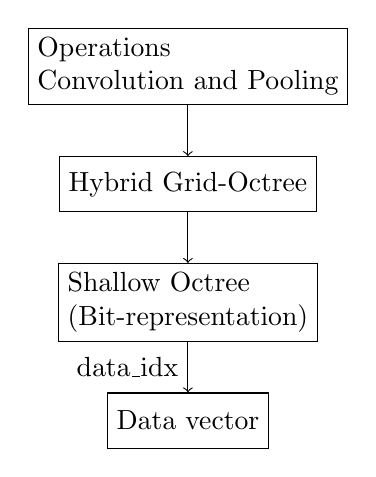
\begin{tikzpicture}[node distance = 1.5cm]
        \node (opt) [brick] {\vbox{\hbox{Operations}\hbox{Convolution and Pooling}}};
        \node (hgo) [brick,below of=opt] {Hybrid Grid-Octree};
        \node (so)  [brick,below of=hgo] {\vbox{\hbox{Shallow Octree}\hbox{(Bit-representation)}}};
        \node (dv)  [brick,below of=so] {Data vector};
        \draw [->] (opt) -- (hgo);
        \draw [->] (hgo) -- (so);
        \draw [->] (so) -- node[left,pos=.5]{data\_idx} (dv);
    \end{tikzpicture}
    \caption{Layers of OctNet}
    \label{fig:octenet:layers}
    \end{figure}

    The OctNet includes two primary part:
    \begin{itemize}
        \item Octree-based data structure for representation.
        \item Optimized convolution-concerned operations for computing.
    \end{itemize}
    The fig.\ref{fig:octenet:layers} shows the details.
    
    \subsection{Vector of data}
    \label{sec:octnet:vd}
    
    The data vector will store the data at leaf-node with a single-D vector.
    
    Let me give an example. The fig.\ref{fig:octnet:bintree} is a binary tree.
    The node, which labled with $0$, means the leaf-node. In other words,
    it will not be split. 
    \begin{figure}
        \centering
        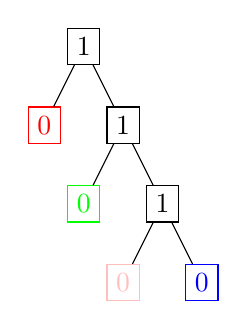
\begin{tikzpicture}[nodes={draw, rectangle},level distance=1cm,sibling distance=1cm]
        \node {1}
        child {node[color=red]{0}}
        child {node{1}
            child {node[color=green]{0}}
            child {node{1}
                child {node[color=pink]{0}}
                child {node[color=blue]{0}}}};
        \end{tikzpicture}
        \caption{A binary tree}
        \label{fig:octnet:bintree}
    \end{figure}
    So the data vector will be fig.\ref{fig:octnet:vd:eg}
    \begin{figure}
         \centering
         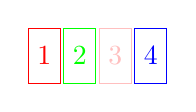
\begin{tikzpicture}[node distance = 0.45cm]
             \node (1) [brick,color=red] {1};
             \node (2) [brick,right of=1,color=green] {2};
             \node (3) [brick,right of=2,color=pink] {3};
             \node (4) [brick,right of=3,color=blue] {4};
         \end{tikzpicture}
         \caption{Example of data vector}
         \label{fig:octnet:vd:eg}
    \end{figure}

    \subsection{Shallow Octree}
    \label{sec:octnet:so}
    
    \citep{DBLP:journals/corr/RieglerUG16} use shallow octree, a full octree, to label shape of octree.
    For a cube, it can be split into octant infinitely. In the shallow octree,
    if a cube is split into octant, it should be labeled with $1$,
    and the leaf-node  will be labeled with $0$, just like fig.\ref{fig:octnet:so}.
    
    \begin{figure}
        \centering
        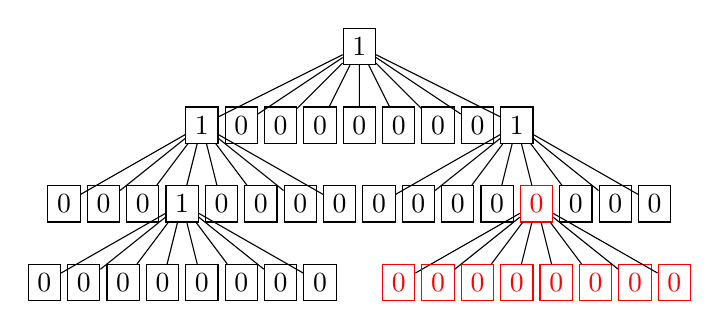
\begin{tikzpicture}[nodes={draw, rectangle},level distance=1cm,sibling distance=0.5cm]
        \node {1}
        child {node{1}
            child {node{0}}
            child {node{0}}
            child {node{0}}
            child {node{1}
                child {node{0}}
                child {node{0}}
                child {node{0}}
                child {node{0}}
                child {node{0}}
                child {node{0}}
                child {node{0}}
                child {node{0}}}
            child {node{0}}
            child {node{0}}
            child {node{0}}
            child {node{0}}}
        child {node{0}}
        child {node{0}}
        child {node{0}}
        child {node{0}}
        child {node{0}}
        child {node{0}}
        child {node{0}}
        child {node{1}
            child {node{0}}
            child {node{0}}
            child {node{0}}
            child {node{0}}
            child {node [color=red]{0}
                child {node [color=red]{0}}
                child {node [color=red]{0}}
                child {node [color=red]{0}}
                child {node [color=red]{0}}
                child {node [color=red]{0}}
                child {node [color=red]{0}}
                child {node [color=red]{0}}
                child {node [color=red]{0}}}
            child {node{0}}
            child {node{0}}
            child {node{0}}};
        \end{tikzpicture}
        \caption{Shallow octree}
        \label{fig:octnet:so}
    \end{figure}
    
    Because the shallow octree is the full octree, for the leaf-nodes which are not at
    the lowest level, these node still have  sub-nodes, just like the nodes marked with red
    in fig.\ref{fig:octnet:so}.
    However, those whose parent nodes are also ``leaf-node'', should be ignored when computing.
    Such representation is called bit-representation.
    
    \subsection{Index funciton}
    \label{sec:octenet:index-func}
    
    \citep{DBLP:journals/corr/RieglerUG16} define a function $I(\cot)$, called \verb|data\_idx|.
    For octree, the $I(\cdot)$ are defined:
    \begin{equation}
        \label{eq:data-index}
        I(i) = 8 \sum\limits_{j=0}^{pa(i)-1}bit(j)+1 - \sum\limits_{j=0}^{i-1}bit(j) + mod(i-1,8)
    \end{equation}
    where $bit(\cdot)$ will return the tree bit-string value at $i$,
    $mod(\cdot)$ denotes modulo operation, and $pa(\cdot)$ will return the parent node's index.
    
    \paragraph{\color{blue}$8 \sum\limits_{j=0}^{pa(i)-1}bit(j)+1$}
    Compute how many nodes are in shallow octree before node $i$.
    
    \paragraph{\color{blue}$-\sum\limits_{j=0}^{i-1}bit(j)$}
    Compute how many nodes are not the lead nodes.
    
    \paragraph{\color{blue}$mod(i-1,8)$}
    Compute offset.
    
    \subsection{Hybrid Grid-Octree}
    \label{sec:octnet:hgo}
    
    The operations of OctNet is not directly done on the tensor or octree,
    but the hybrid grid-octree.
    
    \begin{figure}
        \centering
        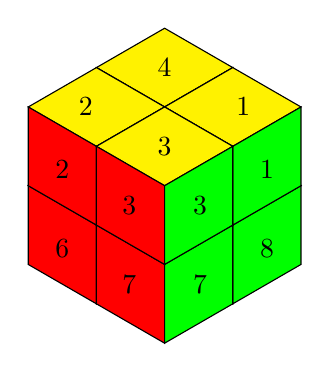
\begin{tikzpicture}
        \cube{0}{0}{0}
        \cube{0}{0}{1}
        \cube{0}{1}{0}
        \cube{0}{1}{1}
        \cube{1}{0}{0}
        \cube{1}{0}{1}
        \cube{1}{1}{0}
        \cube{1}{1}{1}
        \draw (1,1) node {1};
        \draw (-1,1) node {2};
        \draw (0,.5) node {3};
        \draw (0,1.5) node {4};
        \draw (-.45,-0.25) node {3};
        \draw (-.45,-1.25) node {7};
        \draw (-1.3,-.8) node {6};
        \draw (-1.3,0.2) node {2};
        \draw (.45,-0.25) node {3};
        \draw (.45,-1.25) node {7};
        \draw (1.3,-.8) node {8};
        \draw (1.3,0.2) node {1};
        \end{tikzpicture}
        \caption{A cube split into 8 octants.}
        \label{fig:octnet:cube-octant}
    \end{figure}

    A cude(fig.\ref{fig:octnet:cube-octant}) can be split into 8 octants.
    Each of octant can be mapped to a octant on octree(fig.\ref{fig:octnet:octree-1}).

    \begin{figure}
        \centering
        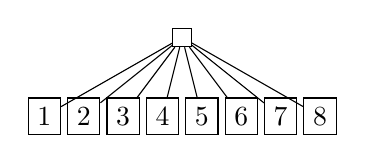
\begin{tikzpicture}[nodes={draw, rectangle},level distance=1cm,sibling distance=0.5cm]
            \node { }
            child {node{1}}
            child {node{2}}
            child {node{3}}
            child {node{4}}
            child {node{5}}
            child {node{6}}
            child {node{7}}
            child {node{8}};
        \end{tikzpicture}
        \caption{A octree for a cube.}
        \label{fig:octnet:octree-1}
    \end{figure}
    
    Since the shallow tree is full-octree, the mapping between hybridgrid-octree
    grid $O(\cdot)$ and shallow octree node $i$ can be easily established.
    In the next subsection, there will be an example of how we use the hybrid 
    grid-octree, data index function, shallow tree and data vector to find out
    the value of a grid in octree.

    \subsection{Example of Hybrid Grid-Octree}
    \label{sec:octnet:eg}
    
    In this subsection, there will be an example of get the value of a octree
    in depth 3 to do convolution operation.
    
    \begin{figure}
        \centering
        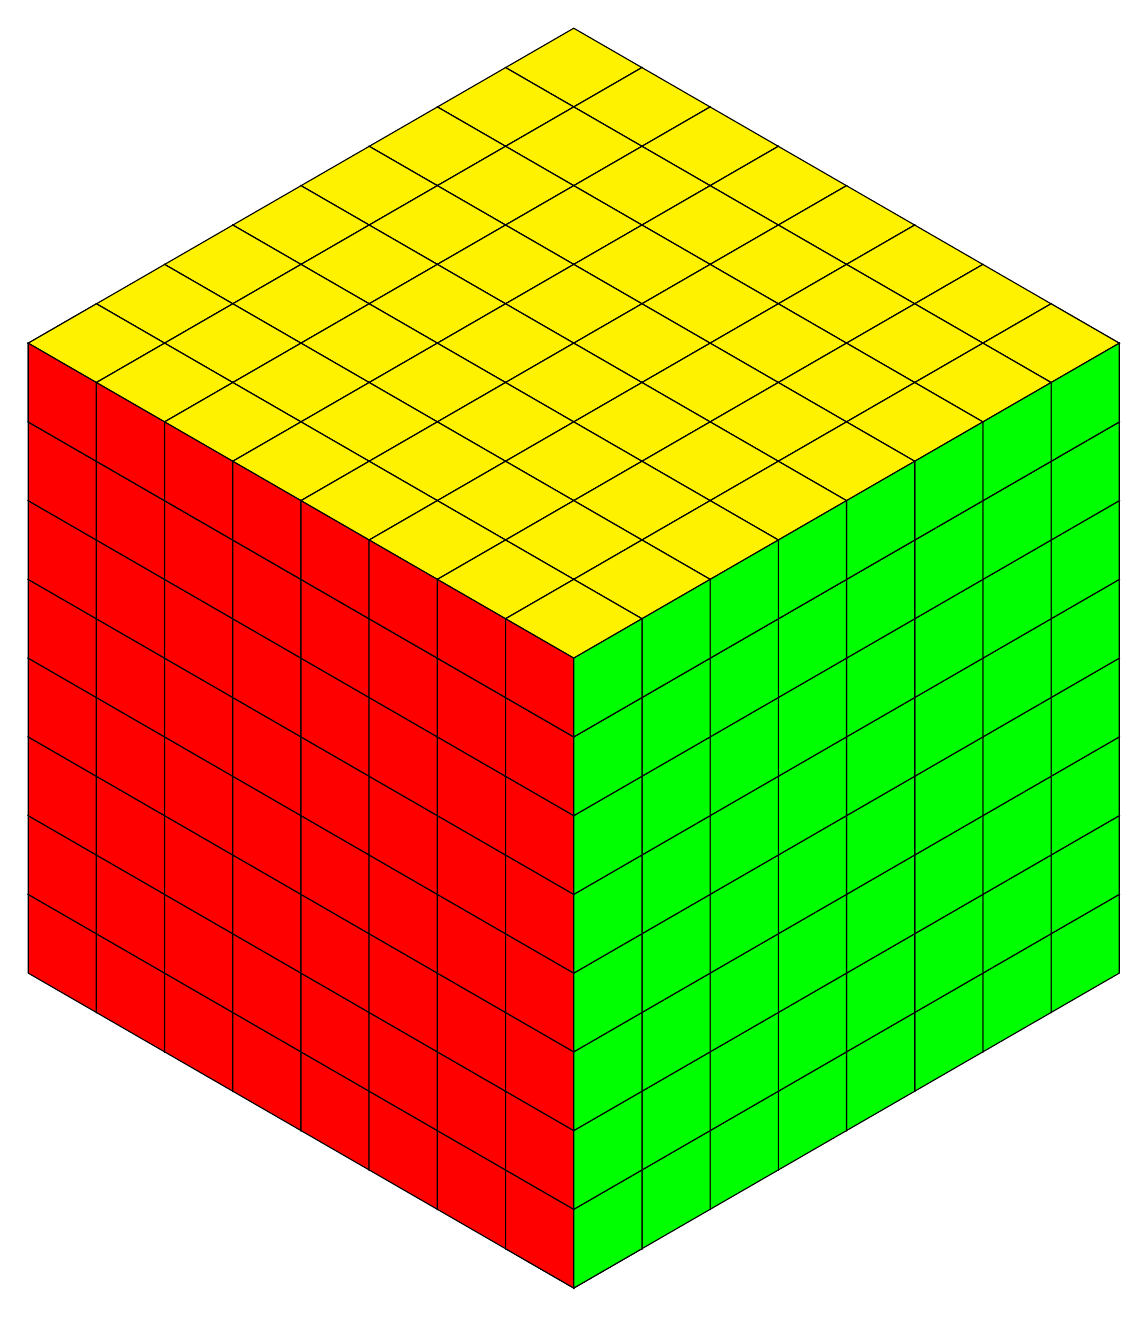
\begin{tikzpicture}
                \foreach \a in {0,...,7}
                    \foreach \b in {0,...,7}
                        \cube{7}{\a}{\b};
                \foreach \a in {0,...,7}
                    \foreach \b in {0,...,7}
                        \cube{\a}{7}{\b};
                \foreach \a in {0,...,7}
                    \foreach \b in {0,...,7}
                        \cube{\a}{\b}{7};
        \end{tikzpicture}
        \caption{A cube in $8^3$ resolution}
        \label{fig:octnet:eg:cude-1}
    \end{figure}

    The octree in depth 3 means the cube with $8^3$ resolution(fig.\ref{fig:octnet:eg:cude-1}).
    
    If we want the value of cude at $(3,4,5)$, the first thing is
    to get this cube's index in shallow tree.
    
    If we use the shown in fig.\ref{fig:octnet:octree-1},
    so index of shallow octree(fig.) is
    \[
      \underbrace{73}_\text{parent node}
    + \underbrace{8 * 8 * (4 - 1)}
    + \underbrace{8 * (7 - 1)}_\text{offset of parent level}
    + \underbrace{(3-1)}_\text{offset} = 315
    \]
    
    \begin{figure}
        \centering
        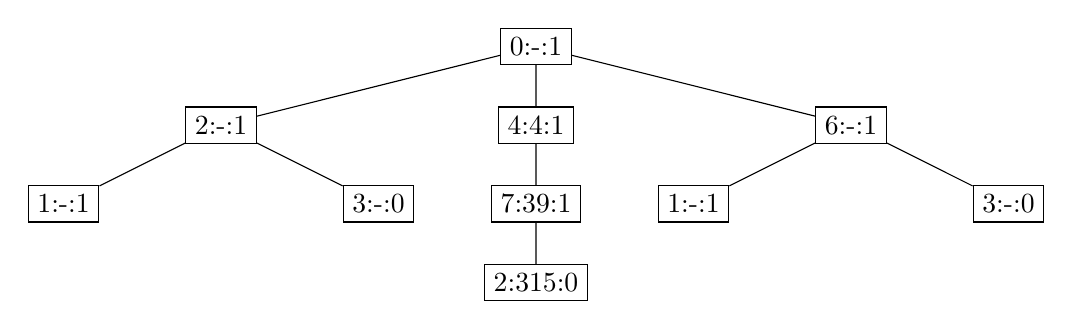
\begin{tikzpicture}[nodes={draw},level distance=1cm,sibling distance=4cm]
        \node {0:-:1}
            child{node{2:-:1}
                child{node{1:-:1}}
                child{node{3:-:0}}
            }
            child {node{4:4:1}
                child {node{7:39:1}
                    child {node{2:315:0}}
                }
            }
            child {node{6:-:1}
                child{node{1:-:1}}
                child{node{3:-:0}}
            }
            ;
        \end{tikzpicture}
        \caption{Shallow octree. In $a:b:c$, a denotes this node is a-th of sub-node, b denotes the index of bit-representation, and c denotes whether
        the node has the sub-nodes. The node $2:315:0$ is the cube in
        fig.\ref{fig:octnet:octree-1} at $(3,4,5)$.}
        \label{fig:octnet:shallowtree}
    \end{figure}

    Then we can use $I(\cdot)$ to compute the index of that cube.
    \begin{align*}
    I(315) &= \underbrace{8 \sum\limits_{j=0}^{pa(315)-1}bit(j)+1}_{\text{nodes above} 315}
           - \underbrace{\sum\limits_{j=0}^{315-1}bit(j)}_{\text{split nodes pre} 315}
           + \underbrace{mod(315-1,8)}_\text{offset}\\
           &= 8 * 5 + 1 - 7 + 2 \\
           &= 36
    \end{align*}
    
    Each node, which is labeled with $1$, there are 8 sub-nodes.
    So for \verb|nodes above|, the number of node before node$315$ is $8$ times of the number
    of the nodes which labeled with $1$.
    
    The \verb|split node| part is about the node do not contain the data, so there should not
    be any space for those node in data vector.
    
    The \verb|offset| is the offset of index.
    
    
    \subsection{Convolutional Operations}
    \label{sec:octnet:co}
    
    \subsubsection{Tensor-based Operations}
    \label{sec:octnet:co:tb}
    
    \paragraph{Convolution}
        \begin{equation}
        \tilde{T}^{(q)}_{i,j,k} = \sum\limits_{p=0}^{P-1} \sum\limits_{l=0}^{L-1} \sum\limits_{m=0}^{M-1} \sum\limits_{n = 0}^{N-1} w_{l,m,n,p,q}T^{(p)}_{\hat{i},\hat{j},\hat{k}}
        \end{equation}
        where $\hat{i} = i -l + \lfloor\frac{L}{2}\rfloor$
    \paragraph{Pooling}
    \begin{equation}
    \tilde{T}_{i,j,k} = \max\limits_{l,m,n \in \left[0,\alpha\right]}T_{\alpha i +l,\alpha j +m,\alpha k +n}
    \end{equation}
    
    \subsubsection{Transform between Tensor-based and Hybrid Grid Octree-based}
    \label{sec:octnet:co:trans}
    
    \paragraph{Hybrid Grid-Octree to Tensor}
        \begin{equation}
        T_{i,j.k} = O[i,j,k]
        \end{equation}
    \paragraph{Tensor to Hybrid Grid-Octree}
        \begin{equation}
        O[i,j,k] = pool\_voxels\left(T_{\overline{i},\overline{j},\overline{k}}\right)
        \end{equation}
        where $pool\_voxels(\cdot)$ is a pooling function, and $(\overline{i},\overline{j},\overline{k})\in \Omega[i,j,k]$
    \paragraph{Transformation of operations from Tensor-based to Hybrid Grid Octree-based}
        \begin{equation}
        g(O)=ten2oc(f(oc2ten(O)))
        \end{equation}
    
    \subsection{Octree-based Operations}
    \label{sec:octnet:oo}
    
    For the octree-based operations, the tensor-based operations are worker
    and octree-based ones are wrapper, just like fig.\ref{sec:octnet:co:tb}    
    
    \begin{figure}
        \centering
        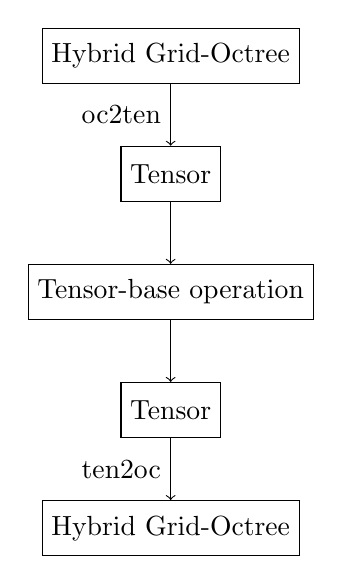
\begin{tikzpicture}[node distance = 1.5cm]
        \node (in) [brick] {Hybrid Grid-Octree};
        \node (in-t) [brick,below of=in] {Tensor};
        \node (f)  [brick,below of=in-t] {Tensor-base operation};
        \node (out-t) [brick,below of=f] {Tensor};
        \node (out)  [brick,below of=out-t] {Hybrid Grid-Octree};
        \draw [->] (in) -- node[left,pos=.5]{oc2ten}(in-t);
        \draw [->] (in-t) -- (f);
        \draw [->] (f) -- (out-t);
        \draw [->] (out-t) -- node[left,pos=.5]{ten2oc} (out);
        \end{tikzpicture}
        \caption{Tensor-based octree operations flowchart.}
        \label{sec:octnet:to-fc}
    \end{figure}

    
    \paragraph{Convolution}
        \begin{eqnarray}
        \tilde{O}[i,j,k] = pool\_voxels(T_{\overline{i},\overline{j},\overline{k}}) \\
        T_{i,j,k} = \sum\limits_{l=0}^{L-1} \sum\limits_{m=0}^{M-1} \sum\limits_{n = 0}^{N-1} w_{l,m,n} O[\hat{i},\hat{j},\hat{k}]
        \end{eqnarray}
    \paragraph{Pooling}
        \begin{equation}
        \tilde{O}[i,j,k] = \begin{cases}
        O[2i,2j,2k] & \text{if\quad} vxd(2i,2j,2k) < lvl \\
        \max\limits_{l,m,n \in \left[0,1\right]}(O[2i +l,2j +m,2k +n]) & \text{else}
        \end{cases}
        \end{equation}
    
    \paragraph{Optimized Convolution operation}
    
        Because of sparse data, so they present a optimized convolutional network(fig.\ref{fig:opt-conv}).
        For a cube, it includes 4 parts:
        \begin{itemize}
            \item constant
            \item corner
            \item edges
            \item face
        \end{itemize}
    
        For the constant, the convolution operation just need to do once.
        For the corner, that just need to 8 times.
        For the edger, it is $(n-2)*12$ times.
        For the face, it is $6(n-2)^2$ times.
        
        \begin{figure}
            \centering
            \includegraphics[width=0.7\linewidth]{../../../image/opt-conv}
            \caption{Optimized convolutional operation.}
            \label{fig:opt-conv}
        \end{figure}
    
    \subsection{Testing Reproduce}
    \label{sec:octnet:test}
    
    I reproduce the testing of ModelNet10 classification task with OctNet 1 ~ 3(fig.\ref{sec:octnet:test:rt}).
    
    \begin{figure}
        \centering
        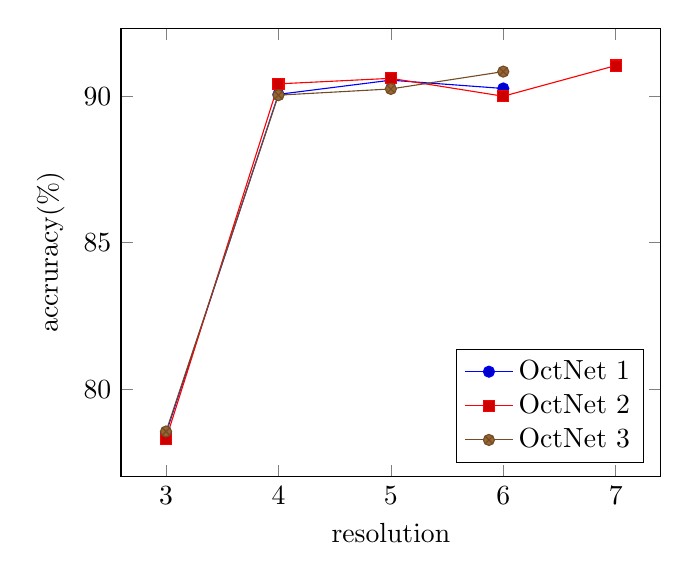
\begin{tikzpicture}
            \begin{axis}[xlabel=resolution,ylabel=accruracy(\%),legend pos = south east]
            \addplot coordinates {
                (3.0,78.49668750000001)
                (4.0,90.06058749999998)
                (5.0,90.54435714285715)
                (6.0,90.26118571428572)
            };\addlegendentry{OctNet 1}
            \addplot coordinates {
                (3.0,78.2902)
                (4.0,90.4185125)
                (5.0,90.6073)
                (6.0,89.99631666666667)
                (7.0,91.04259999999998)
            };\addlegendentry{OctNet 2}
            \addplot coordinates {
                (3.0,78.5517625)
                (4.0,90.0330375)
                (5.0,90.24542857142858)
                (6.0,90.837)
            };\addlegendentry{OctNet 3}
            \end{axis}
        \end{tikzpicture}
        \caption{Testing result}
        \label{sec:octnet:test:rt}
    \end{figure}
    
    \bibliography{../../../random-bib/2-D-CNN%
                 ,../../../random-bib/3d-deep-learning%
                 %
                 }
    \bibliographystyle{plainnat}
\end{document}